\chapter{The Optimality}

\chapterepigraph
{His central result is that the posterior of his universal semimeasure $M$ converges rapidly to the true sequence generating posterior $\mu$, if the latter is computable. Hence, $M$ is eligible as a universal predictor in case of unknown $\mu$.}
{Marcus Hutter, ``On the Existence and Convergence of Computable Universal Priors'' (2003)}

\noindent \textsc{Chapter 4 gave you a prior.} It came from fair coin flips fed to a universal machine: each minimal program whose output begins with $x$, weighted by $2^{-|p|}$, and the weights summed. The universal prior $M(x)$.

You can use $M$. You can also use something else.

The best reason to take $M$ seriously is a theorem.

\section*{The dominance theorem}

Let $\mu$ be any computable probability distribution on output strings: any distribution that an algorithm can sample from, or compute the probability of.\footnote{The theorem in fact holds for the wider class of lower-semicomputable semimeasures, which is the natural home of $M$ itself; ``computable distribution'' is the friendly special case, and the one every example below belongs to.} Most distributions of practical interest are computable. Gaussian, exponential, geometric. Every distribution a statistician writes down with computable parameters. Every distribution a simulation can produce.

The dominance theorem says: there is a constant $c_\mu$ such that

$$M(x) \geq c_\mu \cdot \mu(x)$$

for every string $x$.

In words: for each such $\mu$, $M$ puts at least a fixed fraction of $\mu$'s weight on every string. That fraction can be tiny.

The constant is positive. It does not depend on $x$; it depends on $\mu$ and on the chosen universal machine.

\section*{Why this is true}

The proof is a few lines.

Since $\mu$ is computable, there is a program that reads random bits and generates a sequence distributed according to $\mu$. Write $K(\mu)$ for the length of a shortest description of that generator on the prefix machine of Chapter 4; running the generator on the chosen monotone machine $U$ adds only a fixed overhead, a constant that depends on $U$.

That generator contributes a fixed share of $M$. For any prefix $x$, the fair random inputs that make it begin with $x$ have total weight $\mu(x)$. Encoding the generator costs $K(\mu)+O(1)$ bits, so its share is at least $2^{-K(\mu)-O(1)}\mu(x)$.

Other programs may also contribute, only adding to the total. Therefore

$$M(x) \geq 2^{-K(\mu)-O(1)} \cdot \mu(x).$$

Figure~\ref{fig:dominance-proof} shows the inequality: the $\mu$-sampler's contribution alone, beside the full $M(x)$.

\begin{figure}[h]
\centering
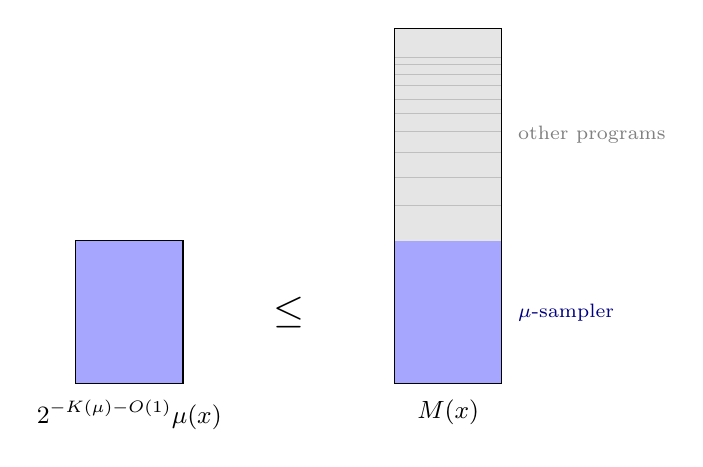
\begin{tikzpicture}[scale=0.9]
  % Bar 1: the μ-sampler's contribution alone
  \draw[thick] (0, 0) rectangle (1.5, 2);
  \fill[blue!35] (0, 0) rectangle (1.5, 2);

  % "≤" between bars
  \node[font=\Large] at (3, 1) {$\leq$};

  % Bar 2: M(x), with μ-sampler portion highlighted at bottom
  \draw[thick] (4.5, 0) rectangle (6, 5);
  \fill[blue!35] (4.5, 0) rectangle (6, 2);
  \fill[gray!20] (4.5, 2) rectangle (6, 5);
  % Internal dividers suggesting many other programs
  \draw[gray!50, thin] (4.5, 2.5) -- (6, 2.5);
  \draw[gray!50, thin] (4.5, 2.9) -- (6, 2.9);
  \draw[gray!50, thin] (4.5, 3.25) -- (6, 3.25);
  \draw[gray!50, thin] (4.5, 3.55) -- (6, 3.55);
  \draw[gray!50, thin] (4.5, 3.8) -- (6, 3.8);
  \draw[gray!50, thin] (4.5, 4.0) -- (6, 4.0);
  \draw[gray!50, thin] (4.5, 4.2) -- (6, 4.2);
  \draw[gray!50, thin] (4.5, 4.35) -- (6, 4.35);
  \draw[gray!50, thin] (4.5, 4.5) -- (6, 4.5);
  \draw[gray!50, thin] (4.5, 4.6) -- (6, 4.6);

  % Labels under bars
  \node[anchor=north, font=\small] at (0.75, -0.1) {$2^{-K(\mu)-O(1)} \mu(x)$};
  \node[anchor=north, font=\small] at (5.25, -0.1) {$M(x)$};

  % Labels to the right of bar 2
  \node[anchor=west, font=\scriptsize, gray] at (6.1, 3.5) {other programs};
  \node[anchor=west, font=\scriptsize, blue!50!black] at (6.1, 1) {$\mu$-sampler};
\end{tikzpicture}
\caption{Why $M$ dominates $\mu$. The bar on the left is the contribution from one program that generates $\mu$, including fixed machine overhead. The bar on the right is the full universal semimeasure $M(x)$, which also includes every other minimal program for $x$. So $M(x)$ is at least the generator's piece alone.}
\label{fig:dominance-proof}
\end{figure}

The construction gives a bound of the form $c_\mu \gtrsim 2^{-K(\mu)}$, with machine-dependent overhead. Distributions that are short to describe can receive a better guarantee; long descriptions can make the guaranteed fraction extremely small. But every lower-semicomputable semimeasure is represented with some positive constant.

\section*{What this means for prediction}

Solomonoff prediction conditions sequential $M$ on observations (Figure~\ref{fig:sequential-prediction}). The observed prefix is fed to $M$; conditional ratios give weights for the next symbol. If the data are generated by a computable probability measure, standard Solomonoff convergence results say these predictions approach the source conditional with probability one, in the senses made precise by the theorem.

\begin{figure}[h]
\centering
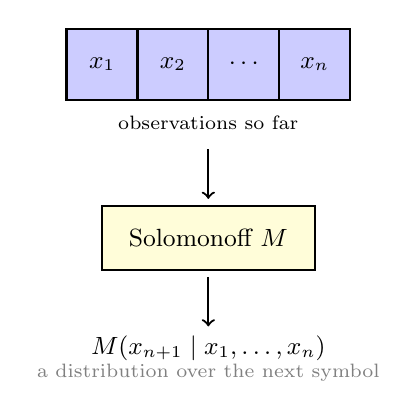
\begin{tikzpicture}[scale=0.9]
  % Input: observed prefix
  \foreach \i/\lbl in {0/{$x_1$}, 1/{$x_2$}, 2/{$\cdots$}, 3/{$x_n$}} {
    \draw[thick, fill=blue!20] (\i, 0) rectangle ({\i+1}, 1);
    \node[font=\small] at ({\i+0.5}, 0.5) {\lbl};
  }
  \node[anchor=north, font=\scriptsize] at (2, -0.1) {observations so far};

  % Arrow down to procedure
  \draw[->, thick] (2, -0.7) -- (2, -1.4);

  % Procedure box
  \draw[thick, fill=yellow!15] (0.5, -2.4) rectangle (3.5, -1.5);
  \node[font=\small] at (2, -1.95) {Solomonoff $M$};

  % Arrow down to output
  \draw[->, thick] (2, -2.5) -- (2, -3.2);

  % Output
  \node[anchor=north, font=\small] at (2, -3.2) {$M(x_{n+1} \mid x_1, \ldots, x_n)$};
  \node[anchor=north, font=\scriptsize, gray] at (2, -3.6) {a distribution over the next symbol};
\end{tikzpicture}
\caption{Sequential prediction. The observed prefix is fed to the procedure; conditional ratios return weights for the next symbol. Under a computable source, Solomonoff's convergence results bring these predictions toward the source conditional.}
\label{fig:sequential-prediction}
\end{figure}

The bound on cumulative log-loss comes directly from the dominance theorem. Take logarithms of the inequality above:

$$\log_2 \mu(x) - \log_2 M(x) \leq K(\mu) + O(1).$$

By the chain rule for log-probabilities, the left side is the cumulative log-loss gap along the sequence. Thus its upper bound is a description-length term plus machine overhead.

The upper bound does not grow with the length of the sequence, and it holds on every sequence, not only on typical ones. Spread over $n$ observations, the guaranteed excess per observation is at most $(K(\mu)+O(1))/n$, which shrinks toward zero. Averaged over sequences drawn from $\mu$, the same gap is a Kullback-Leibler divergence, bounded by the same quantity. Related bounds control cumulative squared prediction error and yield convergence for computable sources. Figure~\ref{fig:dominance} shows the guarantee schematically.

\begin{figure}[h]
\centering
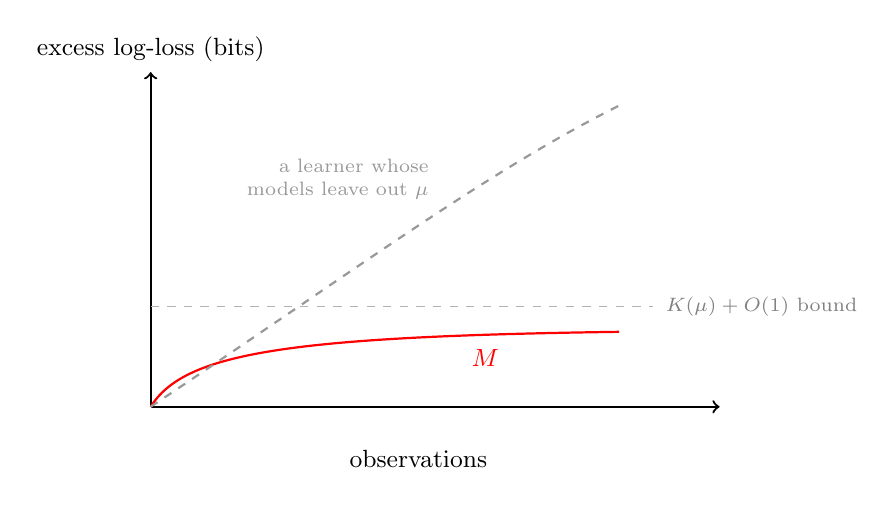
\begin{tikzpicture}[scale=0.85]
  % Axes
  \draw[->, thick] (0, 0) -- (8.5, 0);
  \draw[->, thick] (0, 0) -- (0, 5) node[above, font=\small] {excess log-loss (bits)};

  % Upper-bound line
  \draw[dashed, gray!60] (0, 1.5) -- (7.5, 1.5);
  \node[anchor=west, font=\scriptsize, gray] at (7.55, 1.5) {$K(\mu)+O(1)$ bound};

  % One admissible M trajectory below the bound
  \draw[thick, red] (0, 0) .. controls (0.5, 0.8) and (2, 1.05) .. (7, 1.12);
  \node[anchor=north, font=\small, red] at (5.0, 1.0) {$M$};

  % One illustrative rival trajectory
  \draw[thick, dashed, gray!80] (0, 0) .. controls (3, 2) and (5, 3.5) .. (7, 4.5);
  \node[anchor=east, font=\scriptsize, gray!80, text width=2.6cm, align=right] at (4.3, 3.4) {a learner whose models leave out $\mu$};

  % X-axis label
  \node[anchor=north, font=\small] at (4, -0.5) {observations};
\end{tikzpicture}
\caption{A schematic dominance guarantee. Solomonoff's cumulative log-loss gap has an upper bound of the form $K(\mu)+O(1)$; the red curve is one possible trajectory below it, not a required asymptote. The dashed curve is a learner whose models leave out the source; its excess loss can grow without bound. Many other learners also do well: dominance is a guarantee for $M$, not a ranking of rivals. Spread over more observations, $M$'s guaranteed excess per observation shrinks toward zero.}
\label{fig:dominance}
\end{figure}

This is the central guarantee. Under a computable source, Solomonoff prediction converges while paying a description-dependent overhead. It is a powerful universality result. It is not a claim that $M$ wins at every finite time or under every possible criterion of optimality.

\section*{What this says to the chicken}

Chapter 1 left Russell's chicken on the farm, and Hume's question unanswered. The bound above is the precise, conditional answer that chapter promised.

Write the chicken's life as a sequence: one symbol each morning, food or no food. Suppose the farm runs on some computable rule $\mu$, however elaborate: a hundred mornings of food, or three hundred, and then the morning that is different. Give the chicken $M$ in place of habit. On every possible life, the chicken's total surprise, counted in bits, exceeds the surprise of someone who knew the rule all along by at most $K(\mu) + O(1)$: roughly the length of the shortest description of the farm, plus the machine's constant. If the rule involves no chance, the one who knew it is never surprised at all, and the bound caps the chicken's whole lifetime of surprise.

That is a budget, and it is finite. A Solomonoff chicken can still be surprised on the last morning, and badly. The bound does not say when the surprise comes, and nothing in it protects any particular morning. What it rules out is surprise without limit. However long the chicken lives, the total excess is drawn from a budget fixed by how hard the farm is to describe, not by how long the chicken has been watching.

Notice what has happened to Hume's assumption. The naive answer in Chapter 1 was that the world is uniform, and that answer smuggled in what it set out to prove. The bound needs no uniformity. It needs something else: that the data come from some computable source. That is an assumption too, and no amount of data can establish it. So this is not induction justified from nothing, the thing Hume showed could not be had. It is a different thing: a price for being wrong, stated in advance, on the condition that the source is computable. No chicken can run $M$, which is not computable. The condition and the price hold for the ideal.

\section*{The choice of machine}

The construction of $M$ depended on a choice of universal monotone machine $U$. A different machine $U'$ gives a different prior $M'$.

The invariance theorem says how the choices are related.

For any two universal monotone machines $U$ and $U'$, there exists a constant $c$ such that

$$M(x) \leq c \cdot M'(x) \quad \text{and} \quad M'(x) \leq c \cdot M(x)$$

for all $x$. The constant comes from compiler overhead. If a fixed program of length $\ell$ makes $U$ simulate $U'$, then every run of $U'$ can be reproduced on $U$ for $\ell$ extra bits, so $M(x) \geq 2^{-\ell} M'(x)$; the same argument runs the other way. Mathematics supplies no general ``few hundred bits'' bound for machines chosen in advance.

So universal machines define a multiplicative-equivalence class. This relation supports asymptotic robustness in the computable-source setting. At finite scales, however, the constants may dominate, and a perversely chosen universal machine can encode perverse prior preferences.

There is therefore no single machine-independent prior. There is a family of universal priors with strong asymptotic relations and potentially important finite differences. In any specific construction, you choose a $U$ and keep the choice visible.

\section*{The bedrock, complete}

The bedrock of inference under uncertainty is now in place. Four ingredients:

\begin{itemize}
\item \textbf{Cox-style representation results.} Under stated richness and regularity assumptions, coherent plausibilities can be represented by probability.
\item \textbf{Bayes' theorem.} Conditional probability determines the update once a probability model and prior are supplied.
\item \textbf{Kraft plus fair program bits.} Kraft makes the weights $2^{-|p|}$ admissible on any prefix-free set of programs, the minimal programs for $x$ among them; fair bits choose those weights and, run through a universal monotone machine, define $M$.
\item \textbf{Dominance, convergence, and invariance.} $M$ dominates lower-semicomputable semimeasures up to source- and machine-dependent constants; its predictions converge for computable sources; different universal machines remain multiplicatively related.
\end{itemize}

The results are settled mathematics when their hypotheses stay attached, and together they make $M$ a distinguished ideal for universal prediction. They are not a proof of \emph{the} uniquely rational prior: Kraft permits the short-program preference, fair bits supply it, and dominance gives it a remarkable guarantee. Reading program weights as facts about what exists would be a separate move.

\section*{The bedrock in the wild}

This is mathematics from the 1960s and 1970s, and modern language models have made it culturally visible. They are finite next-token predictors trained to reduce cross-entropy on text, and cross-entropy is cumulative log-loss, the same kind of quantity the bound above controls. That shared quantity is where the analogy is earned, and where it stops: a trained model is not shown to approximate $M$, its training loss charges for the data but not for the length of the model itself, and its performance depends on architecture, optimization, and a fixed compute budget the theorem never mentions. Acting has its own idealization, Hutter's AIXI, introduced in 2000 and developed at book length in 2005: an uncomputable agent that pairs a universal mixture with expected-reward maximization, whose optimality claims depend on the chosen machine, reward, and horizon. The systems illustrate bounded universal prediction. They do not implement it, and they do not confirm the theorem, which was already proved about a different, idealized object.

\section*{Where this leaves you}

The mathematical core is in place: Bayes' theorem, a universal construction, dominance and convergence results, and machine-relative invariance. The distinctions among them matter as much as the formulas.

Chapter 4 called each program a candidate cut. $M$ ranks those candidates by what they cost to write down, and the theorems say how well the ranking predicts. They say what the ranking is good for. What it means is another question.

What remains is interpretation.
